
%----------------------------------------------------------------------------------------
%	PACKAGES AND OTHER DOCUMENT CONFIGURATIONS
%----------------------------------------------------------------------------------------

\documentclass{article}

\usepackage{fancyhdr} % Required for custom headers
\usepackage{lastpage} % Required to determine the last page for the footer
\usepackage{extramarks} % Required for headers and footers
\usepackage[usenames,dvipsnames]{color} % Required for custom colors
\usepackage{graphicx} % Required to insert images
\usepackage{listings} % Required for insertion of code
\usepackage{courier} % Required for the courier font
\usepackage{lipsum} % Used for inserting dummy 'Lorem ipsum' text into the template
\usepackage{amsmath}
\usepackage[a4paper]{geometry}
\RequirePackage[l2tabu, orthodox]{nag}
\usepackage{microtype}
\usepackage{siunitx}
\usepackage{cleveref}
\usepackage[colorlinks=false, pdfborder={0 0 0}]{hyperref}
\usepackage{booktabs}
\usepackage[framed,numbered,autolinebreaks,useliterate]{mcode}

% Margins
\topmargin=-0.45in
\evensidemargin=0in
\oddsidemargin=0in
\textwidth=6.5in
\textheight=9.0in
\headsep=0.25in

\linespread{1.1} % Line spacing

% Set up the header and footer
\pagestyle{fancy}
\lhead{\hmwkAuthorName} % Top left header
\chead{\hmwkClass\ (\hmwkClassInstructor\ \hmwkClassTime): \hmwkTitle} % Top center head
\rhead{\firstxmark} % Top right header
\lfoot{\lastxmark} % Bottom left footer
\cfoot{} % Bottom center footer
\rfoot{Page\ \thepage\ of\ \protect\pageref{LastPage}} % Bottom right footer
\renewcommand\headrulewidth{0.4pt} % Size of the header rule
\renewcommand\footrulewidth{0.4pt} % Size of the footer rule

\setlength\parindent{0pt} % Removes all indentation from paragraphs

%----------------------------------------------------------------------------------------
%	CODE INCLUSION CONFIGURATION
%----------------------------------------------------------------------------------------

\definecolor{MyDarkGreen}{rgb}{0.0,0.4,0.0} % This is the color used for comments
\lstloadlanguages{Perl} % Load Perl syntax for listings, for a list of other languages supported see: ftp://ftp.tex.ac.uk/tex-archive/macros/latex/contrib/listings/listings.pdf
\lstset{language=Perl, % Use Perl in this example
        frame=single, % Single frame around code
        basicstyle=\small\ttfamily, % Use small true type font
        keywordstyle=[1]\color{Blue}\bf, % Perl functions bold and blue
        keywordstyle=[2]\color{Purple}, % Perl function arguments purple
        keywordstyle=[3]\color{Blue}\underbar, % Custom functions underlined and blue
        identifierstyle=, % Nothing special about identifiers                                         
        commentstyle=\usefont{T1}{pcr}{m}{sl}\color{MyDarkGreen}\small, % Comments small dark green courier font
        stringstyle=\color{Purple}, % Strings are purple
        showstringspaces=false, % Don't put marks in string spaces
        tabsize=5, % 5 spaces per tab
        %
        % Put standard Perl functions not included in the default language here
        morekeywords={rand},
        %
        % Put Perl function parameters here
        morekeywords=[2]{on, off, interp},
        %
        % Put user defined functions here
        morekeywords=[3]{test},
       	%
        morecomment=[l][\color{Blue}]{...}, % Line continuation (...) like blue comment
        numbers=left, % Line numbers on left
        firstnumber=1, % Line numbers start with line 1
        numberstyle=\tiny\color{Blue}, % Line numbers are blue and small
        stepnumber=5 % Line numbers go in steps of 5
}

% Creates a new command to include a perl script, the first parameter is the filename of the script (without .pl), the second parameter is the caption
\newcommand{\perlscript}[2]{
\begin{itemize}
\item[]\lstinputlisting[caption=#2,label=#1]{#1.pl}
\end{itemize}
}

%----------------------------------------------------------------------------------------
%	DOCUMENT STRUCTURE COMMANDS
%	Skip this unless you know what you're doing
%----------------------------------------------------------------------------------------

% Header and footer for when a page split occurs within a problem environment
\newcommand{\enterProblemHeader}[1]{
\nobreak\extramarks{#1}{#1 continued on next page\ldots}\nobreak
\nobreak\extramarks{#1 (continued)}{#1 continued on next page\ldots}\nobreak
}

% Header and footer for when a page split occurs between problem environments
\newcommand{\exitProblemHeader}[1]{
\nobreak\extramarks{#1 (continued)}{#1 continued on next page\ldots}\nobreak
\nobreak\extramarks{#1}{}\nobreak
}

\setcounter{secnumdepth}{0} % Removes default section numbers
\newcounter{homeworkProblemCounter} % Creates a counter to keep track of the number of problems

\newcommand{\homeworkProblemName}{}
\newenvironment{homeworkProblem}[1][Problem \arabic{homeworkProblemCounter}]{ % Makes a new environment called homeworkProblem which takes 1 argument (custom name) but the default is "Problem #"
\stepcounter{homeworkProblemCounter} % Increase counter for number of problems
\renewcommand{\homeworkProblemName}{#1} % Assign \homeworkProblemName the name of the problem
\section{\homeworkProblemName} % Make a section in the document with the custom problem count
\enterProblemHeader{\homeworkProblemName} % Header and footer within the environment
}{
\exitProblemHeader{\homeworkProblemName} % Header and footer after the environment
}

\newcommand{\problemAnswer}[1]{ % Defines the problem answer command with the content as the only argument
\noindent\framebox[\columnwidth][c]{\begin{minipage}{0.98\columnwidth}#1\end{minipage}} % Makes the box around the problem answer and puts the content inside
}

\newcommand{\homeworkSectionName}{}
\newenvironment{homeworkSection}[1]{ % New environment for sections within homework problems, takes 1 argument - the name of the section
\renewcommand{\homeworkSectionName}{#1} % Assign \homeworkSectionName to the name of the section from the environment argument
\subsection{\homeworkSectionName} % Make a subsection with the custom name of the subsection
\enterProblemHeader{\homeworkProblemName\ [\homeworkSectionName]} % Header and footer within the environment
}{
\enterProblemHeader{\homeworkProblemName} % Header and footer after the environment
}

%----------------------------------------------------------------------------------------
%	NAME AND CLASS SECTION
%----------------------------------------------------------------------------------------

\newcommand{\hmwkTitle}{Computational Physics} % Assignment title
\newcommand{\hmwkDueDate}{November 20 2015} % Due date
\newcommand{\hmwkClass}{APPLAuSE} % Course/class
\newcommand{\hmwkClassTime}{} % Class/lecture time
\newcommand{\hmwkClassInstructor}{MATLAB - Lu\'is Silva} % Teacher/lecturer
\newcommand{\hmwkAuthorName}{Rog\'erio Jorge} % Your name

%----------------------------------------------------------------------------------------
%	TITLE PAGE
%----------------------------------------------------------------------------------------

\title{
\vspace{2in}
\textmd{\textbf{\hmwkClass:\ \hmwkTitle}}\\
\normalsize\vspace{0.1in}\small{Due\ on\ \hmwkDueDate}\\
\vspace{0.1in}\large{\textit{\hmwkClassInstructor\ \hmwkClassTime}}
\vspace{3in}
}

\author{\textbf{\hmwkAuthorName}}
\date{} % Insert date here if you want it to appear below your name

%----------------------------------------------------------------------------------------

\begin{document}

\maketitle
\thispagestyle{empty}

%----------------------------------------------------------------------------------------
%	TABLE OF CONTENTS
%----------------------------------------------------------------------------------------

\newpage
\tableofcontents
\newpage

%----------------------------------------------------------------------------------------
%	INTRODUCTION
%----------------------------------------------------------------------------------------

\section{Introduction}

Understanding single particle motion dynamics is usually the first step within any plasma physics course. Quoting Francis F. Chen (\textit{Introduction to Plasma Physics and Controlled Fusion}, Springer 1984), plasma has a \textit{schizophrenic} personality, as its densities fall in an intermediate range - collisions may or may not dominate, they depend on the specific process. Hence, charged particle dynamics is important for under-dense plasmas and medium density plasmas. On the other hand, the computational strain provided by particle simulations will depend on the number of particles under consideration.

The objective of this work is to analyse the charged particle motion through the development of a Matlab code. We shall consider a small number of particles as we want a code that runs smoothly in a personal laptop with no parallel computing methods. Typically, we will analyse the behaviour of 10 particles, distributed randomly in a box. There is an imposed external electric and magnetic fields and the interaction between the particles is neglected.

In this case, a charged particle has a circular Larmor gyration plus a drift of the guiding centre. The equation of motion is

\begin{equation}
m\frac{d \vec v}{dt}=q(\vec E+\vec v \times \vec B).
\end{equation}

The cyclotron motion has a frequency $\omega_c$ and a radios $r_L$ around the guiding centre of

\begin{equation}
\omega_c = \frac{q B}{m}, \quad r_L = \frac{v_\perp}{\omega_c}.
\end{equation}

The magnetic field keeps the energy $E = \frac{m v^2}{2}$ constant, so if $\vec B=(0,0,B) \implies v_z=$ constant and $v_\perp=\sqrt{v_x^2+v_y^2}=$ constant. If an additional electric field is present, particles will drift (which means their guiding centre velocity will have a new finite component) with velocity

\begin{equation}
\vec v_E=\frac{\vec E \times \vec B}{B^2}.
\end{equation}

We will only mention one more drift that will be analysed bellow - the Grad-B drift. This drift is usually derived by first order Taylor-expanding the magnetic field about the point $(x_0,y_0,z_0)$ and is given by

\begin{equation}
\vec v_{\nabla B}=v_\perp r_L \frac{\vec B \times \nabla B}{B^2}.
\end{equation}

We considered electron-like particles, as this work is related to solving the equations of motion, illustrating the trajectories and picture the drifts, the different gyrofrequencies and Larmor radius wouldn't add any physical insight.

%----------------------------------------------------------------------------------------
%	MATLAB
%----------------------------------------------------------------------------------------

\section{Matlab Numerical Code}

As Matlab allows the use of different files as single functions, the code was divided into 8 scripts

\begin{itemize}
\item Lorentz - serves as ``input file'' and initialization. Ask the user if he wants a quick test (all the necessary homework plotting) or a customized test.
\item Lorentz\_Bfield - function to evaluate the magnetic field at each point. It allows a uniform $B$ on $z$, a sinusoidal and a $1/z$ variation.
\item Lorentz\_dsolve - differential equation solver, either with 4th order Runge-Kutta or Euler method
\item Lorentz\_main - initializes position, velocity, energy and error vectors and calls the different functions defined above. At the end of the evaluation it writes to an hdf5 file the results.
\item Lorentz\_MBDist\_histogram - using the initial velocity assigned in Lorentz\_main, evaluates if the temperature is being assigned correctly by fitting to a 1-D Maxwell-Boltzmann distribution.
\item Lorentz\_plot - taking the title, labels and plot name as an input, it renders the graphics in a ``publishable'' quality.
\item Lorentz\_video - after solving for the trajectories, creates a loop of plots that saves everything inside a high quality \textit{.mp4} video. It also saves the last plot as a \textit{.pdf} file.
\item Lorentz\_visualize - plots the trajectory of the particles and defines the axis of the plot.
\end{itemize}

As input we allow the user after calling the function Lorentz to specify:

\begin{itemize}
\item Number of particles
\item Particle temperature - in Kelvin
\item Magnetic field on $z$ - either uniform, cosine or $1/r$ variation
\item Electric field - constant vector on an arbitrary direction
\item Solver - Runge-Kutta or Euler
\item Plane - 2D plot in the $xy, yz, xz$ plane or in 3D
\item Number of steps - total number of time units to numerically simulate.
\end{itemize}

Afterwords, having defined the electron mass, charge and Boltzmann's constant, we use as timestep and characteristic length

\begin{equation}
dt=0.01 \times \frac{2 \pi}{\omega_c},\quad L=10 \times \frac{v_{th}}{\omega_c}, \quad v_{th}=\sqrt{\frac{2 k_B T}{m}}.
\end{equation}

All the resulting movies, figures and hdf5 files are stores in the folder ``Results''.

%----------------------------------------------------------------------------------------
%	Diagnostics
%----------------------------------------------------------------------------------------

\section{Diagnostics}

\subsection{Code Verification}

In order to verify the implementation of the Lorentz force solver, we look in Fig. 1 to the trajectories of 10 particles with an uniform magnetic field on the $z$ direction with and without an uniform electric field on the $y$ direction. It is seen on both cases the gyromotion of particles around a $B$ field line in the $z$ axis and in the second case a particle drift velocity in the $x$ axis. We also see the random distribution of particles in the box with all sides equal to $L$ and different particle initial velocity.

\begin{figure}[h!]
  \centering
    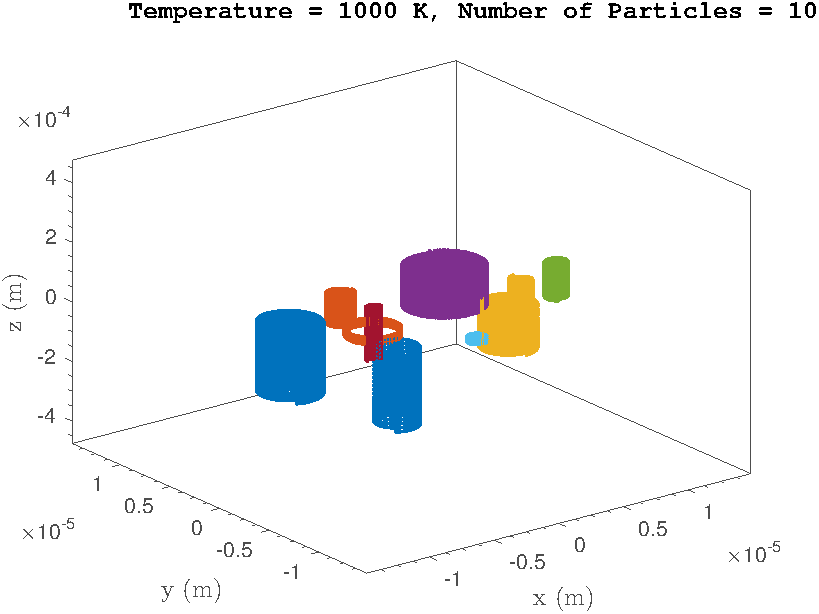
\includegraphics[width=0.49\textwidth]{../Results/Lorentz_xyz_RK4_unifB_E0_10particles.pdf}
    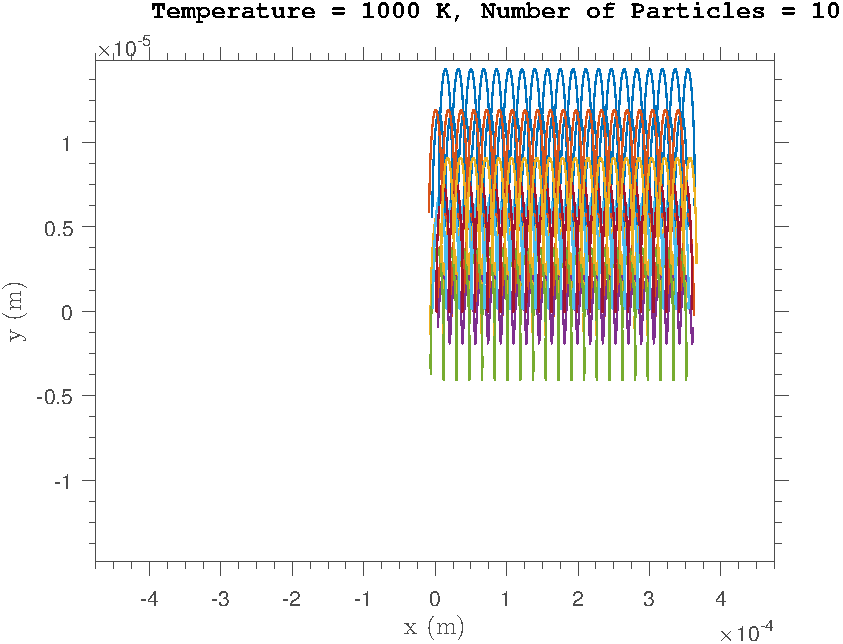
\includegraphics[width=0.49\textwidth]{../Results/Lorentz_xy_RK4_unifB_E5_10particles.pdf}
    \label{test1}
  \caption{Left: Particle trajectory with uniform $B$ field and no $E$ field. Right: Uniform $E$ field in the $y$ direction causes a drift in the $x$ direction.}
\end{figure}

To verify that particles are correctly initialized with a specific temperature, we take the initial velocity on a specific direction and perform a non-linear fit to a Gaussian distribution function in Fig. 2. This allows us to analyse the standard deviation $\sigma$ and mean $\mu$, comparing with the Maxwell-Boltzmann 1-D distribution with $\sigma_{MB}=v_{th}$ and $\mu_{MB}=0$. The accuracy of this analysis depends on the number of particles used, so we perform a test with a greater set of particles that the rest of the diagnostics.

\begin{figure}[h!]
  \centering
    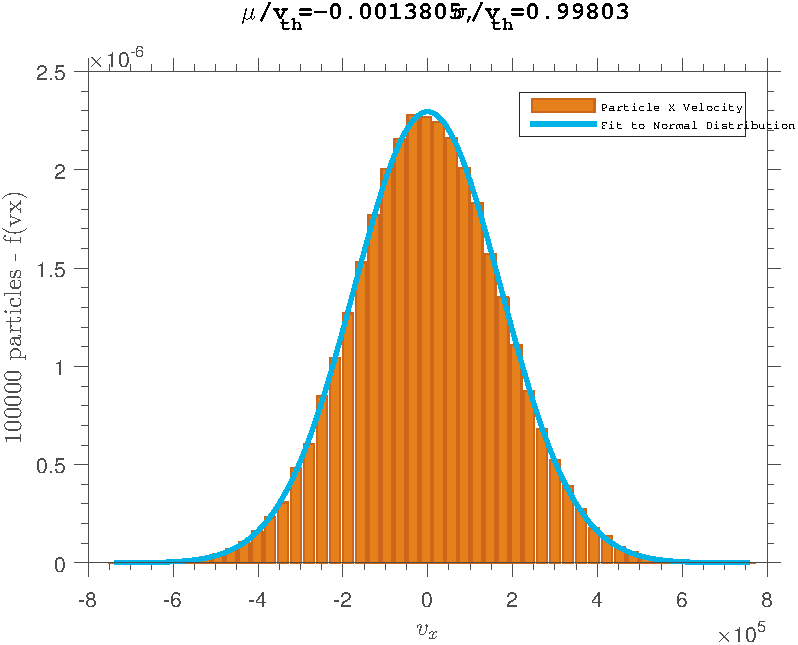
\includegraphics[width=0.49\textwidth]{../Results/Distribution_unifB_E0_100000particles.pdf}
    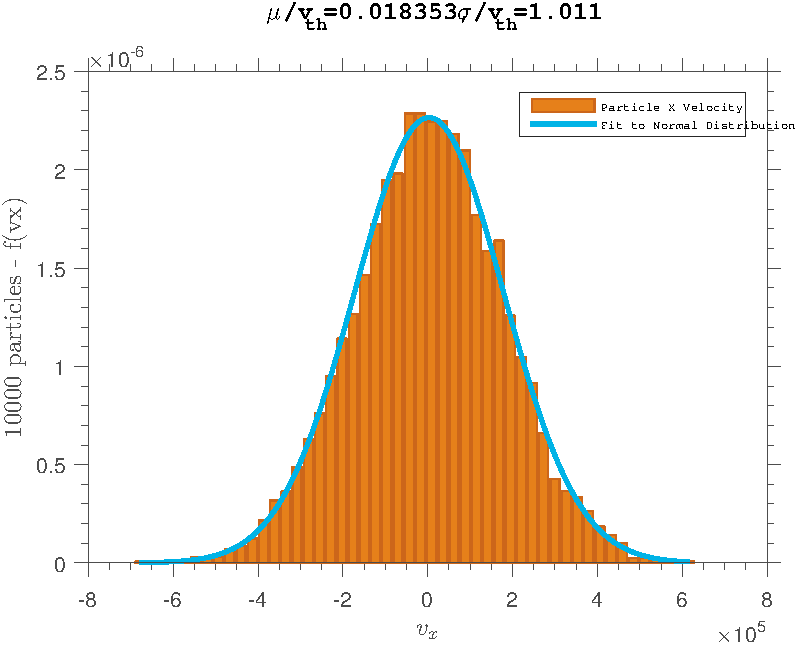
\includegraphics[width=0.49\textwidth]{../Results/Distribution_unifB_E0_10000particles.pdf}
    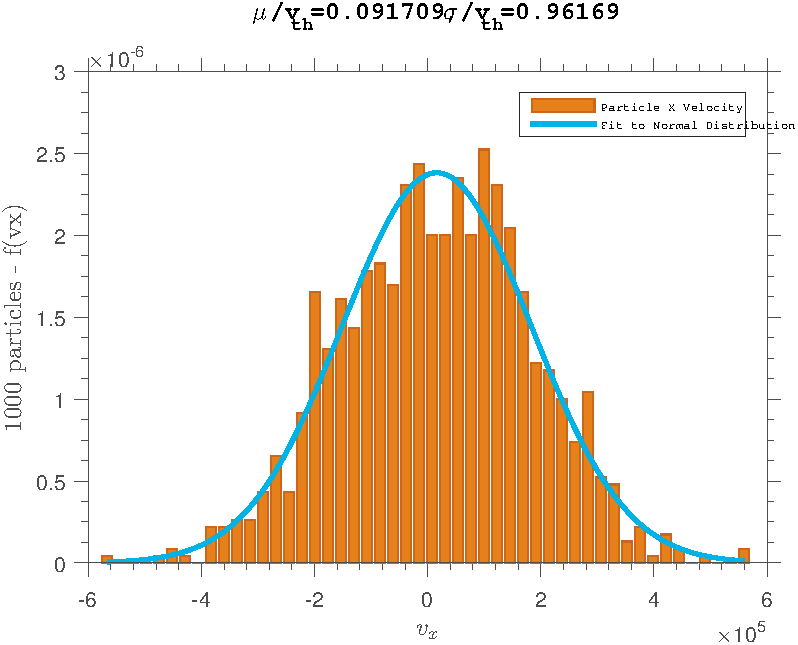
\includegraphics[width=0.49\textwidth]{../Results/Distribution_unifB_E0_1000particles.pdf}
    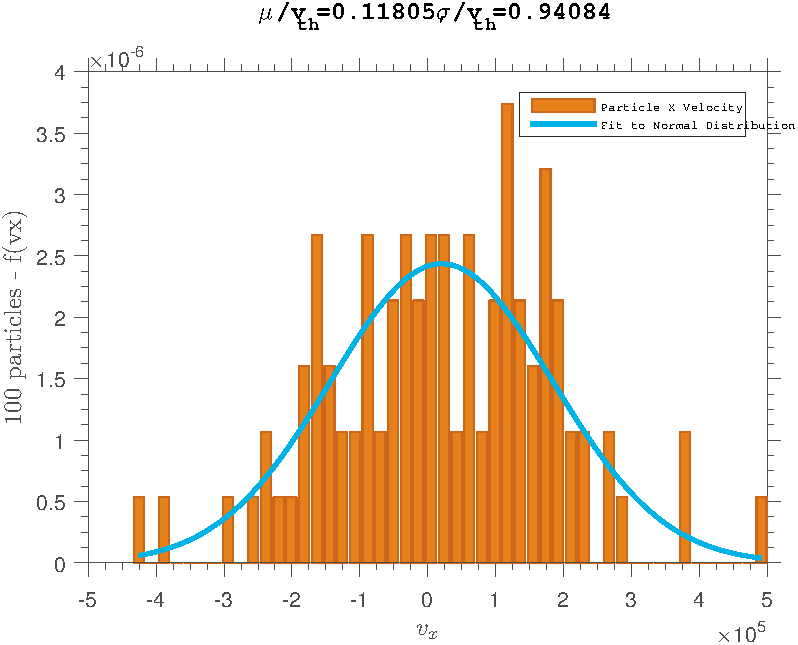
\includegraphics[width=0.49\textwidth]{../Results/Distribution_unifB_E0_100particles.pdf}
    \label{dist}
  \caption{Histogram of the initial particle velocity and resulting non-linear fit to a Gaussian distribution. Fit parameters (mean $\mu$ and standard deviation $\sigma$) displayed.}
\end{figure}

\subsection{Differential Solver Comparison}

In the section, we shall use a result discussed in the introduction: if we only have an uniform stationary magnetic field, the energy is conserved. If we had a perfect numerical method, this would be true. Unfortunately, a small error determining the numerical velocity at a specific timestep introduces an error in the energy. A good numerical method should minimize this error, so to compare both methods we look at the relative error

\begin{equation}
\epsilon(t)=\frac{|E(t)-E_0|}{E_0},
\end{equation}

\noindent where $E$ is the energy and $E_0 = E(t=0)$. We can clearly see in Fig. 3 that the relative error with Runge-Kutta is several orders of magnitude smaller than with the Euler one.

\begin{figure}[h!]
  \centering
    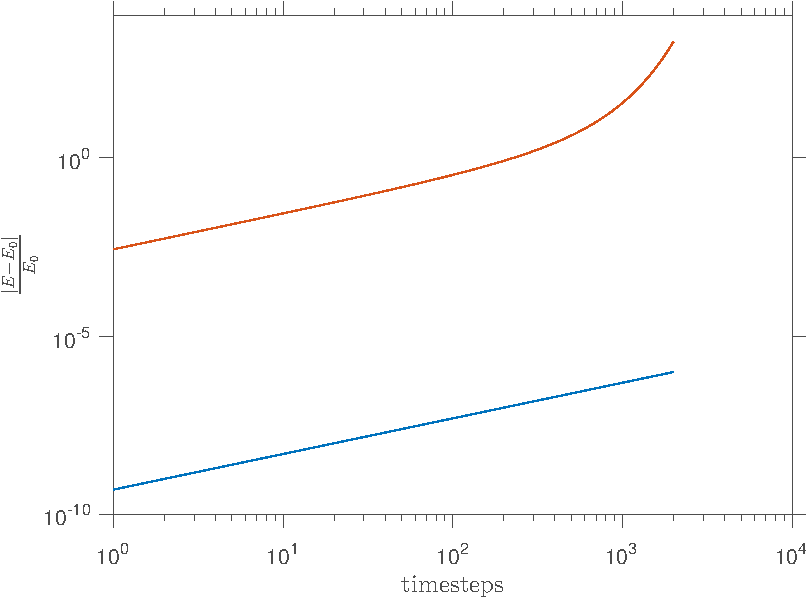
\includegraphics[width=0.49\textwidth]{../Results/energy_error_both.pdf}
    \label{err}
      \caption{Comparison between differential solvers. The red line is the relative energy error with the Euler method and the blue line with the 4th order Runge-Kutta one.}
\end{figure}

\subsection{Particle Drifts}

As the code allows the use of an arbitrary (constant) electric field and an arbitrary magnetic field, we can look at the two drifts discussed in the introduction - the $E \times B$ drift and the Grad-B one. The particle trajectories are illustrated in Fig. 4. The uniform electric field that leads to the observed drift is of the form

\begin{equation}
\vec E = (0,E_0,0),
\end{equation}

\noindent where we used $E_0 = 5$ kV/cm. To observe the Grad-B drift, the implemented B field is of the form

\begin{equation}
\vec B = (0,B_0 \cos \frac{2 \pi y}{L},0).
\end{equation}

This means that particles shall drift in the positive or negative $x$ direction depending on the initial $y$ position of each particle, as we see on Fig. 4.

\begin{figure}[h!]
  \centering
    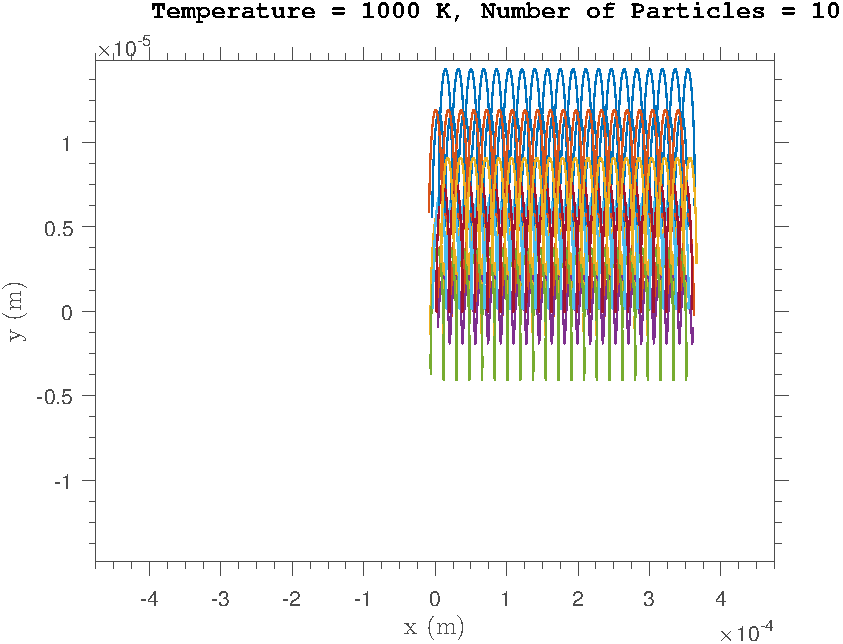
\includegraphics[width=0.49\textwidth]{../Results/Lorentz_xy_RK4_unifB_E5_10particles.pdf}
    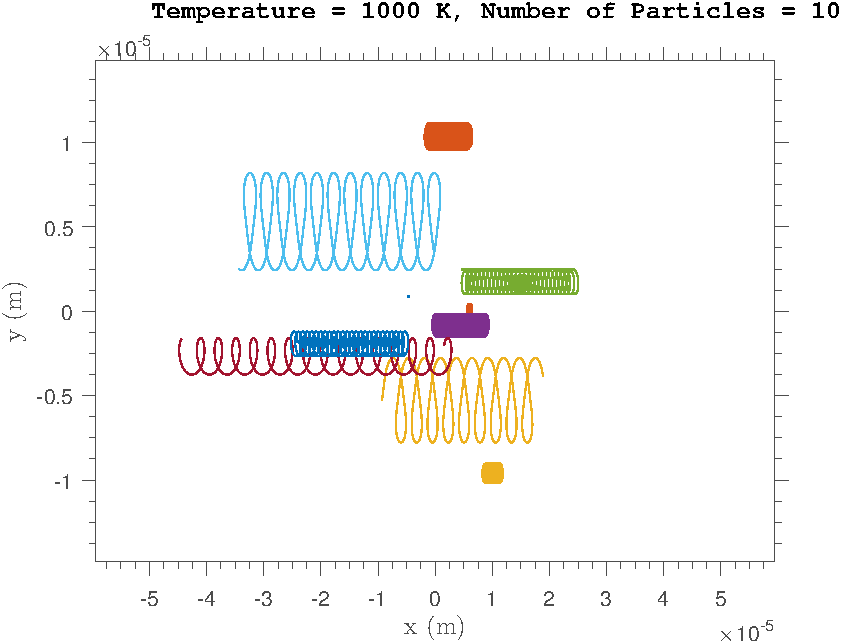
\includegraphics[width=0.49\textwidth]{../Results/Lorentz_xy_RK4_cosB_E0_10particles.pdf}
    \label{drift}
      \caption{Left: Analysis of $E \times B$ drift to the right. Right: Grad-B drift with direction dependent on the positive or negative $y$ position of the particle.}
\end{figure}

%----------------------------------------------------------------------------------------
%	CONCLUSION
%----------------------------------------------------------------------------------------

\section{Conclusion}

The code was developed during the week of 16 - 20 of November within the Advanced Computational Physics Course (Matlab module). The two objectives were achieved: start a Matlab code from scratch and understand the specific software operations (matrix multiplication, ODE solver, function and variable definition, ...) and analyse single charged particle motion with the same code. We have also seen how important numerical methods are in numerical simulations. As seen in Fig. 5, with the Euler method the Larmor radius of the particles increases over time, which is not physical in this scenario.

\begin{figure}[h!]
  \centering
    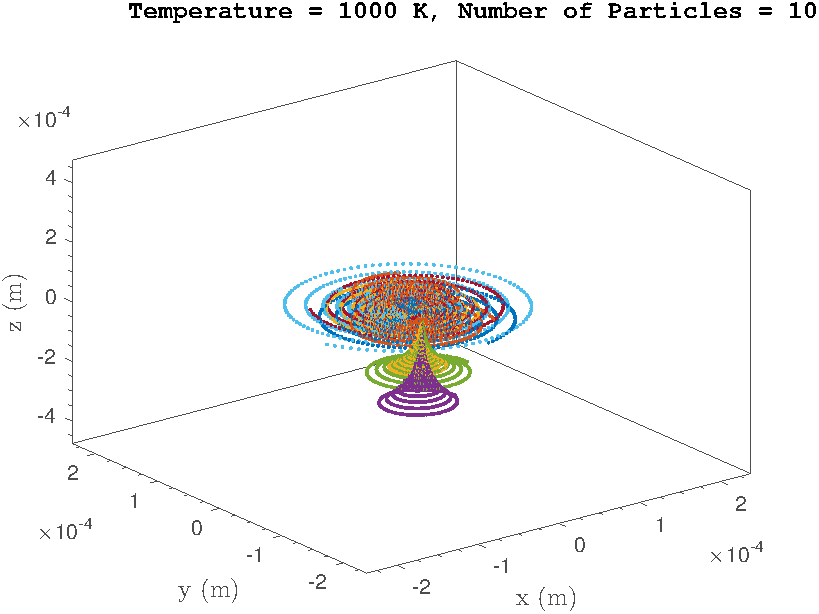
\includegraphics[width=0.49\textwidth]{../Results/Lorentz_xyz_Euler_unifB_E0_10particles.pdf}
    \label{}
      \caption{Larmor radius increase due to numerical error with Euler method.}
\end{figure}

It allows the user to visualize in 2 our 3 dimensions, specify the number of particles, initial temperature and electromagnetic profiles. Furthermore, the timestep and characteristic lengths are internally defined so to resolve at the gyrofrequency and Larmor radius scales.

As a next step, the inclusion of particle-particle interactions through a simple Coulomb term should be straightforward to implement due to the simplicity of the ODE solver (defined in a specific script). The next challenge would be to implement a Poisson solver, where the electric and magnetic fields would depend on particle dynamics and we would have to resort to Maxwell's equations.

%----------------------------------------------------------------------------------------

\end{document}